% 2009 年浙江卷理科第 20 题：四棱锥 P-ABC 型立体图（平面 PAC⊥平面 ABC）。
% 来源 PDF：普通高考/2009/2009浙江理.pdf，SHA-256 8b9a62d8af65c0049a04b2c462e5bc8dc66a464244ca2c2462c6cdfafc5c2d89。
% 原页：第 2 页第 1 栏中部，书页码 566。
% 重绘依据：A 在左、C 在右、B 在前下方，P 在 AC 中垂面上；E∈PA、F∈PB、
%   O 为 AC 中点、G 为 OC 中点。实线为可见棱 PA、PB、PC、AB、BC 与 BE；
%   虚线为 AC（过 O）、BO、EO、FG。
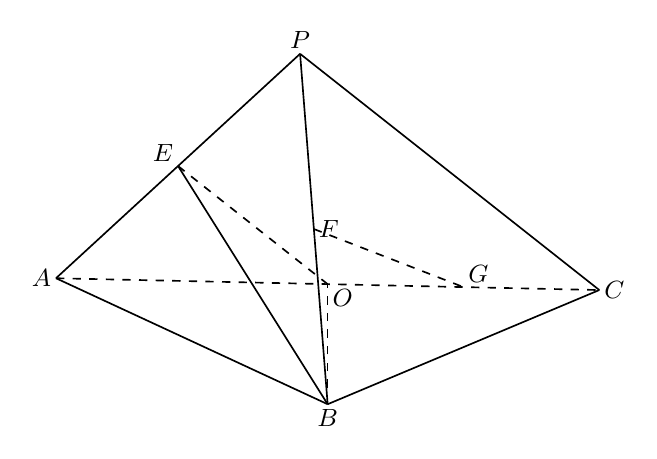
\begin{tikzpicture}[semithick, every node/.style={inner sep=1.5pt, font=\small}]
  \coordinate (P) at (3.1,4.6);
  \coordinate (A) at (0,1.75);
  \coordinate (C) at (6.9,1.60);
  \coordinate (O) at (3.45,1.675);
  \coordinate (B) at (3.45,0.15);
  \coordinate (E) at (1.55,3.175);
  \coordinate (F) at (3.275,2.375);
  \coordinate (G) at (5.175,1.6375);

  \draw (P) -- (A);
  \draw (P) -- (B);
  \draw (P) -- (C);
  \draw (A) -- (B);
  \draw (B) -- (C);
  \draw (E) -- (B);

  \draw[dashed] (A) -- (C);
  \draw[dashed] (B) -- (O);
  \draw[dashed] (E) -- (O);
  \draw[dashed] (F) -- (G);

  \node[above] at (P) {$P$};
  \node[left] at (A) {$A$};
  \node[below] at (B) {$B$};
  \node[right] at (C) {$C$};
  \node[above left] at (E) {$E$};
  \node[right] at (F) {$F$};
  \node[above right] at (G) {$G$};
  \node[below right] at (O) {$O$};
\end{tikzpicture}
